\section{Pigmented Skin Lesions}\label{sec:chp1sec2}

Pigmented skin lesions or melanocytic nevi appear on the surface of the skin~\cite{kaufman2005melanoma}, where the melanocyte cells grow in clusters beside the normal skin cells. 
This is a natural transformation of skin cells and creates benign \ac{psls} such as: 

%\begin{figure}[ht]
%\centering
%		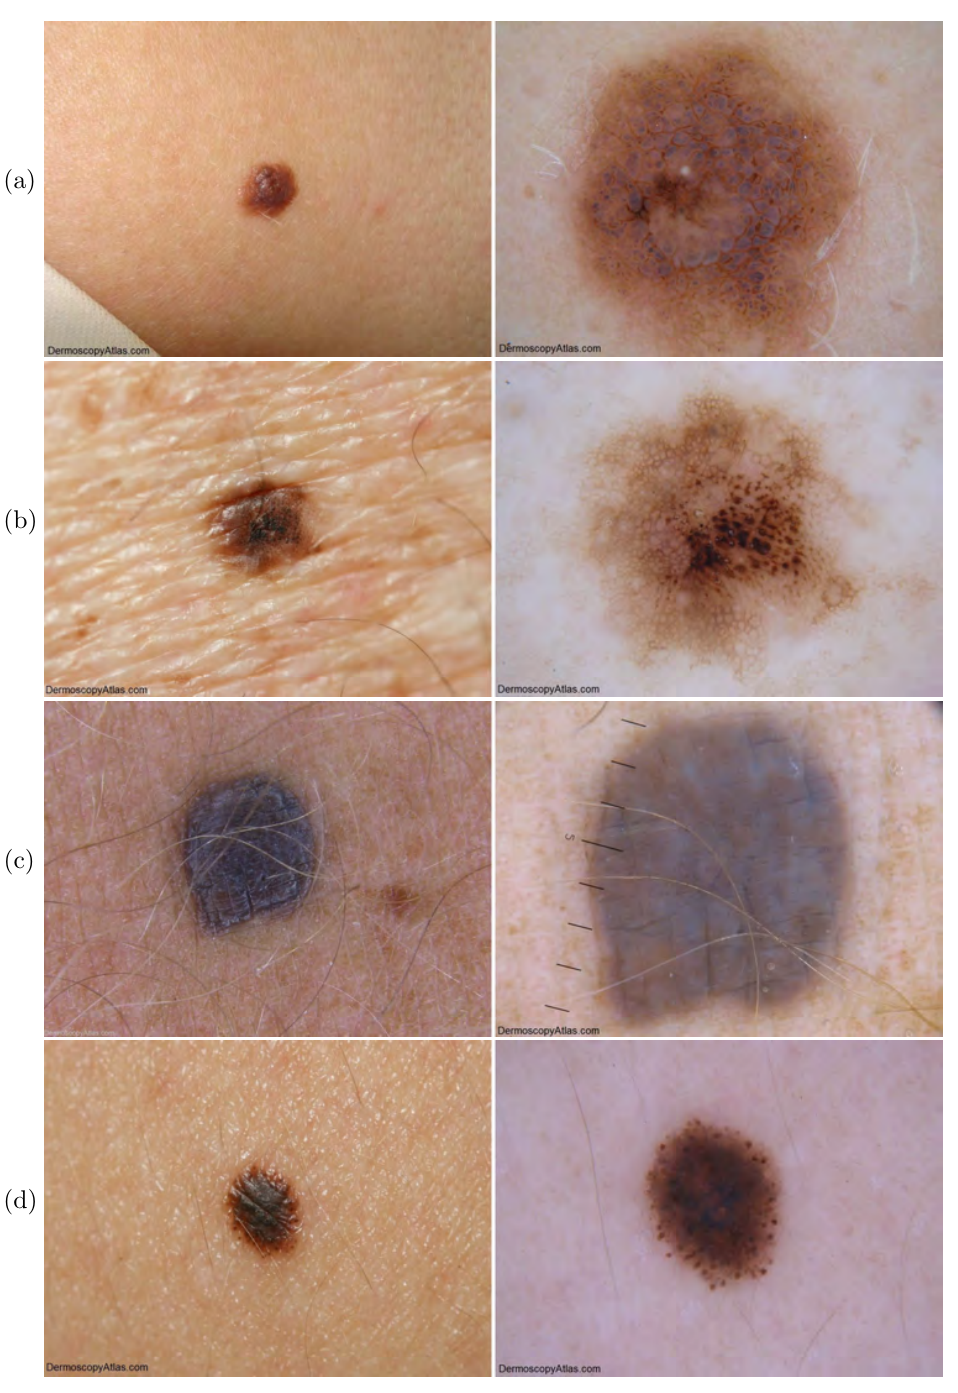
\includegraphics[width = 0.6\textwidth]{Chapter1/Figures/Clinical_DP.png}	
%	\caption{Images of pigmented skin lesions, right column represent the cinical images and left dermoscopy images are presented: (a) congenital nevus; (b) dysplastic nevus; (c) blue nevus; (d) Spitz nevus. {\color{red} ask for permission}}
%		\label{fig:PSLs}
%\end{figure}

\begin{description}
   \item [Freckle] or ephelis are pale-brown macular lesions which are usually of less than 3 \si{\milli\meter} diameter with a poorly defined lateral margin \cite{newton2010lentigos}. 
% which appears and darkens on light-exposed skin sites if  being exposed to ultraviolet
   \item [Common nevi] which are typical flat melanocytic nevi or moles.
   \item [Congenital nevi] which are moles that appear at birth, also known as ``birth marks''.
   \item [Atypical or dysplastic nevi] are common nevi with inconsistent coloration, irregular edges, blurry borders, scale-like texture and a diameter greater than 5 \si{\milli\meter} ~\cite{kaufman2005melanoma}. 
Atypical mole syndrome or dysplastic nevus syndrome, describes individuals with large quantities of dysplastic nevi. 
Such individuals face a higher risk of developing melanoma (6 to 10 times greater than other people with few nevi)~\cite{newton2010lentigos}. 
However, only a small number of these dysplastic nevi might develop into melanoma and most dysplastic nevi will never become cancer.

  \item [Blue nevi] are melanocytic nevi comprised of abnormal collections of benign pigment melanocytes located in the dermis rather than at the dermoepidermal junction~\cite{newton2010lentigos}.
The blue or blue-black appearance of the lesion is caused by light reflection of melanin in the dermis.  
  \item [Pigmented Spitz nevi] are uncommon benign nevi that share a similar physical characteristics to melanoma and are usually seen in children~\cite{newton2010lentigos}. 

\end{description}

From the aforementioned lesions, congenital and dysplastic nevi are most likely to develop into malignant melanoma~\cite{friedman1985early}.  


 
 %%% {I dont know if it is necessary to include this or not} Atypical mole syndrome, also known as “Familial Atypical Multiple Mole Melanoma” (FAMMM) or dysplastic nevus syndrome, describes individuals with large quantities of atypical nevi and possibly inherited melanomas. The relative risk of developing a melanoma in such individuals is around 6 to 10 times that of people with very few nevi [5].



%%% Local Variables: 
%%% mode: latex
%%% TeX-master: "../thesis"
%%% End: 